\section{Natural numbers as grammar}
\index{natural numbers|(}
Math in early history (early childhood) is counting.  Count 
pebbles or beads and give the patterns names
\begin{center}
    $0\defeq$ \underline{\hspace{5mm}}, 
    $1\defeq$ \StrokeOne,
    $2\defeq$ \StrokeTwo,
    $3\defeq$ \StrokeThree,
    $4\defeq$ \StrokeFour,
    $5\defeq$ \StrokeFive,...
\end{center}
One hypothesis for the symbol
``0'' is that it looks like the shape left by removing the last pebble from
a sand table leaving behind no pebbles.

\index{Peano}
It struck Giuseppe Peano in the early 1900's that tallies would be easier to get
right mathematically than digits. With the following two rules Peano introduced
the natural numbers to the formalism of math.
\begin{quote}
    \textit{
    $N_0$ vale ``numero'', et es nomen commune de 0,1,2, etc.\\
    $0$ $\to$  ``zero''\\
    $+$ $\to$ ``plus''.  Si $a$ es numero, $a+$ indica ``numero sequente $a$''.
    }
\end{quote}
% It is fitting that the Italian is in italics.
(See G. Peano \emph{Formulaire de mathematiques.~I-V}, p.27.)
Replacing $+$ with \StrokeOne ~(and equating \StrokeFive$\defeq$\StrokeFour~\StrokeOne),
Peano's model of numbers is simply the grammar of tallies.

Today notation has evolved.  These numbers are now almost always designated as
\emph{natural numbers} and denoted $\mathbb{N}$.  Instead of $a+$ we now often
write $S~k$  or $S(k)$ calling it the ``successor'' to the natural number $k$.  
Programming however has held closer to the original with notation like 
\code{i++} and \code{++i}.

\index{tag}\index{token}\index{\code{<Token>}}\index{\code{::=}}\index{Walrus}
We mentioned Peano was merely recording a grammar.  Today we write grammars with
list of rules, called \emph{production rules}.  Some rules are to specify what
makes up the alphabet of symbols in our grammar.  For Peano, $0$ and $S$ are the
complete alphabet.  So we may write either $0$ on its own, or we may pre-pend
the symbol $S$ to any existing natural number.  Each rule is given a name called
a \emph{token} (or \emph{tag}) and denoted \code{<Name>}. Since the Walrus
$\defeq$ is our assignment of variables (more on this later), we use the
``astonished Walrus'' $::=$ as assignment of production rules.   Taken together
the grammar is the following, shown next to the childhood grammar for tallies.
\begin{center}
\begin{minipage}{0.4\textwidth}
\begin{Gcode}[]
<Nat> ::= 0 
<Nat> ::= S <Nat>
\end{Gcode}
\end{minipage}
\hfill
\begin{minipage}{0.45\textwidth}
\begin{Gcode}[]
<Tally> ::=  
<Tally> ::= | <Tally>
\end{Gcode}
\end{minipage}
\end{center}
In the first rule we are told \code{0} is a natural number, denoted
\code{0:Nat}, just as any whitespace can start a tally. We say that the natural
number grammar \emph{accepts} \code{0} because it matched some production rule,
and the Tally grammar accepts whitespace, usually denoted $\epsilon$.  In the
second rule if we encounter an \code{S} it must be followed by an \emph{already
known} natural number.  So \code{S0:Nat} but \code{0S} would not be accepted as
it is not found as a production rule.  Going forward we use $\mathbb{N}$ 
for \code{Nat} and the usual name $0,1\defeq S0, 2\defeq SS0,\ldots$ as is common.
We retain the notation $n:\mathbb{N}$, instead of $n\in \mathbb{N}$, on account 
of the view that we need natural numbers well before we have a notion of Set Theory.

\index{language}
\begin{definition}
    The words (also called strings) of letters accepted by a grammar is called
    the grammar's \emph{language}.
\end{definition}

\begin{example}
The natural numbers are the language of Peano's grammar, that is, the language of tallies.
\end{example}

The significance of the ``already known'' clause of the rules is to prevent ambiguity 
with terms like $n=$\code{SSS....} where the \code{S} continue forever.
For if we remove one \code{S} form this $n$, the string is unchanged (thanks to 
the infinite number of $S$'s).  Since we are engaged in deciding if $n$ is a natural number and its substring 
is $n$, it is not of the form \code{S k} for \code{k:Nat}.  Hence the grammar 
rejects such an $n$.  Grammar's like these are called \emph{primitive recursive}
meaning that the recursion can only depend backwards 
in history.

\begin{definition}
    A production rule that appears more than once is called \emph{inductive}.
\end{definition}

An accepted short hand for inductive productions rules is to name it once 
and separate the cases by $\mid$, for instance,
\begin{center}
\code{<Nat>::= 0 | S <Nat>} \\
\begin{Gcode}[]
<Nat> ::= 0 
        | S <Nat>
\end{Gcode}
\end{center}
Because of this notation for inductive types I will hence forth limit my use of tallies
to avoid confusion, but I stress that a simplicity often emerges from thinking 
of tallies instead of successors.
    

\begin{remark}
    Some argue that $0$ does not belong in $\mathbb{N}$ because 
    we begin counting at $1$.  Others argue that Peano's postulates
    clarify that $0$ is a natural number and begin counting from there.
    % Both perspectives have a point but neither is correct.  
    It is the case that $0$ is a natural number (even by a different symbol 
    it will behave as $0$).  At the same time notice every count is 
    a tally, so it begins at 1, not 0, that is $a+$, $S$, \code{++i} are
    counts.  Therefore it is a misunderstanding of numbers to omit $0$ 
    from $\mathbb{N}$ and it as much a misunderstanding treat $0$ as the first count.
\end{remark}

\subsection{Drawings of grammar}
For each accepted word we can associate a graph where the nodes are the
production rule used at that stage to accept the fragment of the string, and
edges are any data needed by that rule to accept the substring.  This is called
the \emph{parse graph}.  In our cases they will always be trees so they are
often called \emph{parse trees}\index{parse tree} but you may also hear them
called \emph{abstract syntax trees} or ``ASTs''.\index{AST}\index{abstract
syntax tree}  In this example $0$ depends on nothing but $S$ depends on an
existing symbol.  Here are the first three parse trees in boxes.
\begin{center}
    \begin{tikzpicture}
    
    \node[draw] (A) at (0,0) {\begin{tikzpicture}
        \node (0) at (0,0) {0};
    \end{tikzpicture}};

    \node[draw] (B) at (3,0) {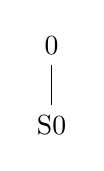
\begin{tikzpicture}
        \node (0) at (0,0) {0};
        \node (S0) at (0,-1) {S0};
        \draw[-] (0) -- (S0);
    \end{tikzpicture}};

    \node[draw] (C) at (6,0) {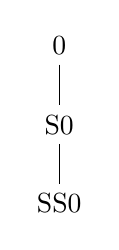
\begin{tikzpicture}
        \node (0) at (0,0) {0};
        \node (S0) at (0,-1) {S0};
        \node (SS0) at (0,-2) {SS0};
        \draw[-] (0) -- (S0);
        \draw[-] (S0) -- (SS0);
    \end{tikzpicture}};
    
    \draw[->] (A) edge["S"] (B);
    \draw[->] (B) edge["S"] (C);
    \draw[dashed,->] (C) edge["S"] (9,0);
\end{tikzpicture}
\end{center}
Between these boxes we have a different graph, the graph that 
plots how one production rule evolves an existing string to another.
This outside graph we call the \emph{word graph}.\index{word graph}  We often condense 
the parse trees to a string to draw the word graph compactly.
\begin{center}
    \begin{tikzpicture}
        \node (0) at (0,0) {0};
        \node (1) at (3,0) {S0};
        \node (2) at (6,0) {SS0};
        \coordinate (3) at (9,0);
        \draw[thick,->] (0) edge["S"] (1);
        \draw[thick,->] (1) edge["S"] (2);
        \draw[dashed,thick,->] (2) edge["S"] (3);
    \end{tikzpicture}
\end{center}

\subsection{Realizing grammar}

We do well to acknowledge inductive types of data as basic programs. Computers
understand this much. Listing~\ref{lst:peano} shows two programs you could run
today that implement Peano's idea. There are of course many differences.
Visibly, the left-hand side favors mathematically minded symbolic notation and
economizes even on parentheses in the spirit of ``$\sin x$'' notation. Meanwhile
the right-hand side favors a verbose imitation of natural language and prefers
the $\sin(x)$ notation.  Set the differences aside.

\begin{lstfloat}
\begin{center}
\begin{minipage}{0.37\textwidth}
\begin{Fcode}[]
data Nat = Z 
    | S (k:Nat)

zero = Z
two = S (S zero)
\end{Fcode}
\end{minipage}
\hfill
\begin{minipage}{0.62\textwidth}
\begin{Pcode}[language=Sava]
class Nat
  case Zero() extends Nat
  case Next(k:Nat) extends Nat
sealed  // no more cases
zero = new Zero()
two = new Next(new Next(zero))
\end{Pcode}
\end{minipage}
\end{center}
\caption{Peano's natural numbers programmed in two different programming languages.}
\label{lst:peano}
\end{lstfloat}
    

Even without a deep understanding of these programs, one can make out the
contours of Paeno's definitions.  Both use a mix of keywords (in blue) to tell
our system to prepare a new type (or class) of data that will be called
\code{Nat}.  Then they instruct the system to accept exactly two ways to make
such data. It may be some initial state, \code{Z}, respectively \code{Zero},
that depends on nothing; otherwise, we must give data \code{k} of type
\code{Nat}, denoted \code{k:Nat}, which will then produce new data \code{S k},
respectively \code{Next(k)}.  In many systems the keyword \code{new} is 
used to help clue the reader into the fact that this is some data being now 
created.  It helps remind us that numbers do not  exists on their own, 
we have to expend resources (energy \& storage) to create them. 


